\documentclass[11pt]{article}
\usepackage[utf8]{inputenc}
\usepackage[english]{babel}
\usepackage{bilal2vec}

\title{SE 380 — HW 1}
\author{Bilal Khan\\
\href{mailto:bilal2vec@gmail.com}{bilal2vec@gmail.com}}
\date{\today}

\begin{document}

\maketitle

\tableofcontents

\section{1}

\subsection{a}

\[ x = \begin{bmatrix} x_1 \\ x_2 \end{bmatrix} = \begin{bmatrix} \theta \\ \dot{\theta} \end{bmatrix} \]
\[ u = \tau \]
\[ J \ddot{\theta} + \dfrac{mgl}{2} \sin \theta = \tau \]

\[ J \ddot{\theta} + \dfrac{mgl}{2} \sin \theta = u \]

\begin{align*}
    \begin{bmatrix}
        \dot{x_1} \\
        \dot{x_2} \\
    \end{bmatrix}
    &=
    \begin{bmatrix}
        x_2 \\
        \dfrac{u}{J} - \dfrac{mgl}{2J} \sin x_1 \\
    \end{bmatrix}
\end{align*}

With the required approximation of $\sin x = x$ to show this in matrix form, this is given by:

\[ \dot{x}(t) = A x(t) + Bu(t) \]

\[
\begin{bmatrix}
    \dot{x_1}(t) \\
    \dot{x_2}(t) \\
\end{bmatrix}
=
\begin{bmatrix}
    0 & 1 \\
    - \dfrac{mgl}{2J} & 0 \\
\end{bmatrix}
\begin{bmatrix}
    x_1(t) \\
    x_2(t) \\
\end{bmatrix}
+
\begin{bmatrix}
    0 \\
    \dfrac{1}{J} \\
\end{bmatrix}
u(t)
\]

\subsection{b}

The system is at its equilibrium points when $\dot{x}(t) = 0$. Therefore, we have that 

\[
\dot{x}(t) = 
\begin{bmatrix}
    0 \\
    0 \\
\end{bmatrix}
=
\begin{bmatrix}
    \dot{\theta} \\
    \ddot{\theta} \\
\end{bmatrix}
\]

Plugging this into our original equation, we have that

\[ J (0) + \dfrac{mgl}{2} \sin \theta = u \]
\[\sin\theta = \dfrac{2u}{mgl} \]

Equilibrium will happen at all points where $\sin \theta = \frac{2u}{mgl}$

\subsection{c}

The system is at an equilibrium point for state $\bar{x} = \begin{bmatrix} 0 \\ 0 \\ \end{bmatrix}$ and and input $\bar{u} = 0$.

We can linearalize the system around this point by taking the Jacobian of $\dot{x}$ with respect to $x$ and $u$.

\[
    A = 
    \begin{bmatrix}
        \dfrac{\partial \dot{x_1}}{\partial x_1} & \dfrac{\partial \dot{x_1}}{\partial x_2} \\
        \dfrac{\partial \dot{x_2}}{\partial x_1} & \dfrac{\partial \dot{x_2}}{\partial x_2} \\
    \end{bmatrix}
    = \begin{bmatrix}
        0 & 1 \\
        - \dfrac{mgl}{2J} \cos x_1 & 0 \\
    \end{bmatrix}
    = \begin{bmatrix}
        0 & 1 \\
        - \dfrac{mgl}{2J} \cos (0) & 0 \\
    \end{bmatrix}
    = \begin{bmatrix}
        0 & 1 \\
        - \dfrac{mgl}{2J} & 0 \\
    \end{bmatrix}
\]

\[
    B =
    \begin{bmatrix}
        \dfrac{\partial \dot{x_1}}{\partial u} \\
        \dfrac{\partial \dot{x_2}}{\partial u} \\
    \end{bmatrix}
    = \begin{bmatrix}
        0 \\
        \dfrac{1}{J} \\
    \end{bmatrix}
\]

The linearalized system is given by the general expression

\[ \dot{x} \approx \dot{x}(\bar{x}, \bar{u}) + A (x - \bar{x}) + B (u - \bar{u}) \]
\[ \dot{x} \approx A(x) + B (u) \]
\[
    \dot{x} \approx
    \begin{bmatrix}
        0 & 1 \\
        - \dfrac{mgl}{2J} & 0 \\
    \end{bmatrix}
    x +
    \begin{bmatrix}
        0 \\
        \dfrac{1}{J} \\
    \end{bmatrix}
    u
\]

\subsection{d}

The system is at equilibrium for $\bar{x} = \begin{bmatrix} \pi / 4 \\ 0 \\ \end{bmatrix}$ and $\bar{u} = \dfrac{mgl}{2\sqrt{2}}$.

We can again linearalize the system around this point by taking the Jacobian of $\dot{x}$ with respect to $x$ and $u$.

\[
    A =
    \begin{bmatrix}
        \dfrac{\partial \dot{x_1}}{\partial x_1} & \dfrac{\partial \dot{x_1}}{\partial x_2} \\
        \dfrac{\partial \dot{x_2}}{\partial x_1} & \dfrac{\partial \dot{x_2}}{\partial x_2} \\
    \end{bmatrix}
    = \begin{bmatrix}
        0 & 1 \\
        - \dfrac{mgl}{2J} \cos x_1 & 0 \\
    \end{bmatrix}
    = \begin{bmatrix}
        0 & 1 \\
        - \dfrac{mgl}{2J} \cos (\pi / 4) & 0 \\
    \end{bmatrix}
    = \begin{bmatrix}
        0 & 1 \\
        - \dfrac{mgl}{2J \sqrt 2} & 0 \\
    \end{bmatrix}
    = \begin{bmatrix}
        0 & 1 \\
        - \dfrac{mgl}{2 \sqrt 2 J} & 0 \\
    \end{bmatrix}
\]

\[
    B =
    \begin{bmatrix}
        \dfrac{\partial \dot{x_1}}{\partial u} \\
        \dfrac{\partial \dot{x_2}}{\partial u} \\
    \end{bmatrix}
    = \begin{bmatrix}
        0 \\
        \dfrac{1}{J} \\
    \end{bmatrix}
\]

The linearalized  system is given by the general expression

\[ \dot{x} \approx \dot{x}(\bar{x}, \bar{u}) + A (x - \bar{x}) + B (u - \bar{u}) \]
\[ \dot{x} \approx A(x - \bar{x}) + B (u - \bar{u}) \]
\[
    \dot{x} \approx
    \begin{bmatrix}
        0 & 1 \\
        - \dfrac{mgl}{2 \sqrt 2 J} & 0 \\
    \end{bmatrix}
    (x - \bar{x}) +
    \begin{bmatrix}
        0 \\
        \dfrac{1}{J} \\
    \end{bmatrix}
    (u - \bar{u})
\]

\subsection{e}

The system is at equilibrium at part (c) and at part (d) when it is at a 45 degree angle with the horizontal so I would use part (c)'s linearalized system to approximate the behavior of the system around the equilibrium point close to its initial conditions and part (d)'s linearlization when it is in equilibrium close to its initial conditions.

\section{2}

\subsection{a}

\begin{minted}{python}
    import numpy as np
    import matplotlib.pyplot as plt

    def sim(delta_t, T, l, x, u):
        t = 0
        path = [x[:2]] # store p_x and p_y for bike path

        while t <= T:
            p_x, p_y, theta, v, delta = x[0], x[1], x[2], x[3], x[4]
            a, w = u(t)
            x_dot = np.array([
                v * np.cos(theta),
                v * np.sin(theta),
                (v / l) * np.tan(delta),
                a,
                w
            ])

            x = x + delta_t * x_dot
            t = t + delta_t

            p_x_prime, p_y_prime = x[0], x[1]
            path += [[p_x_prime, p_y_prime]]
        
        return np.array(path)
\end{minted}

\subsection{b}

\begin{minted}{python}
    import numpy as np
    import matplotlib.pyplot as plt

    delta_t = 0.01
    T = 10
    l = 2
    x = np.zeros(5)
    u = lambda t: (0.1, np.cos(t))

    path = sim(delta_t, T, l, x, u)
    
    plt.plot(path[:, 0], path[:, 1], label="Bike kinematic dynamics")
    plt.title("Path of bicycle")
    plt.xlabel("p_x")
    plt.ylabel("p_y")
    plt.legend()
    plt.show()
\end{minted}

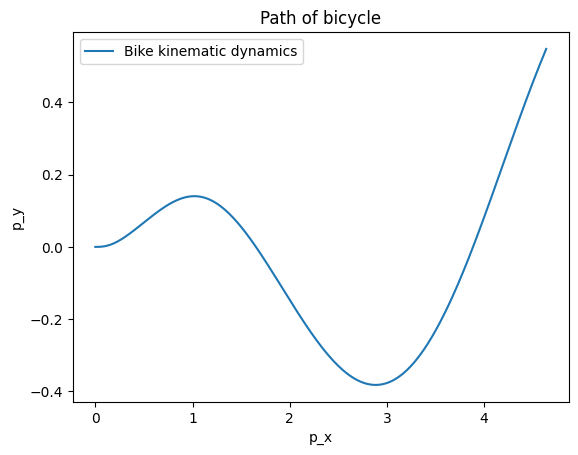
\includegraphics{a1.png}

\end{document}
